% =====================================================================
%  WCCM 2026 / ECCOMAS — MS090E, 22 July 2026.
%  PAPER-FAITHFUL deck: follows the Frontiers in Materials 2025 paper
%  (and the English slides 27-44 of nishioka_progress_20260114.pptx).
%  Extension (architecture sweep / variants) appears ONLY as a brief
%  outlook teaser — co-author-safe, per supervisor's instruction.
%  Build: latexmk -pdf wccm_beamer_paper.tex  (needs biber)
% =====================================================================
\documentclass[aspectratio=169,10pt]{beamer}

\usetheme{metropolis}
\usecolortheme{default}

\usefonttheme{professionalfonts}
\usepackage[T1]{fontenc}
\usepackage[utf8]{inputenc}
\usepackage{newtxtext,newtxmath}
\usepackage[protrusion=true,expansion=true]{microtype}  % thesis-grade typography

\usepackage{booktabs}
\usepackage{amsmath,amssymb}
\usepackage{graphicx}
\usepackage{xcolor}
\usepackage{tikz}
\usetikzlibrary{positioning,arrows.meta}
\usepackage{array}

\usepackage[style=numeric-comp,sorting=none,backend=biber,maxnames=2,giveninits=true]{biblatex}
\addbibresource{refs_submission.bib}
\renewcommand*{\bibfont}{\scriptsize}
\AtEveryCite{\scriptsize\color{luhblue}}

\definecolor{luhblue}{RGB}{21,101,192}
\definecolor{alertred}{RGB}{198,40,40}
\definecolor{okgreen}{RGB}{27,94,32}
\setbeamercolor{frametitle}{bg=luhblue, fg=white}
\setbeamercolor{progress bar}{fg=luhblue}
\setbeamercolor{alerted text}{fg=alertred}
\setbeamercolor{example text}{fg=okgreen}
\metroset{progressbar=frametitle, block=fill}

\usepackage{multicol}

% tiny source-attribution footer on every content slide (very light, bottom).
% (Our own Frontiers paper is attributed here, NOT cited as prior work in-text.)
\setbeamertemplate{footline}{%
  \hbox{}\vspace{1pt}%
  \hbox to \paperwidth{\hskip2mm
    {\tiny\color{gray!70!black} Nishioka \textit{et al.}, Front.\ Mater.\ \textbf{12}:1652484 (2025)}%
    \hfill
    {\tiny\color{gray!70!black}\insertframenumber}\hskip2mm}%
  \vspace{2pt}}

\graphicspath{{figures_paper/}{../results/}}
\newcommand{\best}[1]{{\color{okgreen}\textbf{#1}}}

\title{Development of a Defect Estimation Method for CFRP Interstage
Structures with Holes using Finite Element Analysis and Graph Neural Networks}
\author[K.\ Nishioka et al.]{\underline{Keisuke Nishioka}\inst{1} \and Yuta Kojima\inst{2}
\and Toshiya Saito\inst{3} \and Masahito Washiya\inst{3}
\and Kosuke Kawakami\inst{3} \and Mayu Muramatsu\inst{4}}
\institute{\inst{1}Keio University, Sci.\ for Open \& Environ.\ Systems \quad
\inst{2}Nagoya University \\ \inst{3}JAXA, R\&D Directorate \quad
\inst{4}Keio University, Mech.\ Engineering}
\date{17th WCCM / ECCOMAS 2026, Munich \quad MS090E}

% =====================================================================
\begin{document}

{\setbeamertemplate{footline}{}\maketitle}
\note{Faithful to the Frontiers 2025 paper. Headline result: macro-F1 61\% with GAT
on surface DSPSS. Keep the architecture extension as a single outlook slide.}

% ---------------------------------------------------------------------
\begin{frame}{Introduction: CFRP in space transportation}
\begin{columns}[T]
\begin{column}{0.56\textwidth}
  \vspace{0.3em}
  CFRP carries primary load in reusable launch vehicles
  (high specific strength)~\cite{CFRP_Hou2019,cfrp_aerospace1}.

  \vspace{0.6em}
  \textbf{Interlaminar delamination} around bolt holes critically degrades
  integrity, especially under repeated use. Reliable \emph{defect
  localization} is essential.

  \vspace{0.6em}
  Conventional NDT — ultrasonic~\cite{ultrasonic_air1}, X-ray
  CT~\cite{xray1}, tap testing~\cite{tap_auto1} — is costly and
  operator-dependent~\cite{defect_review}.
\end{column}
\begin{column}{0.44\textwidth}
  \centering
  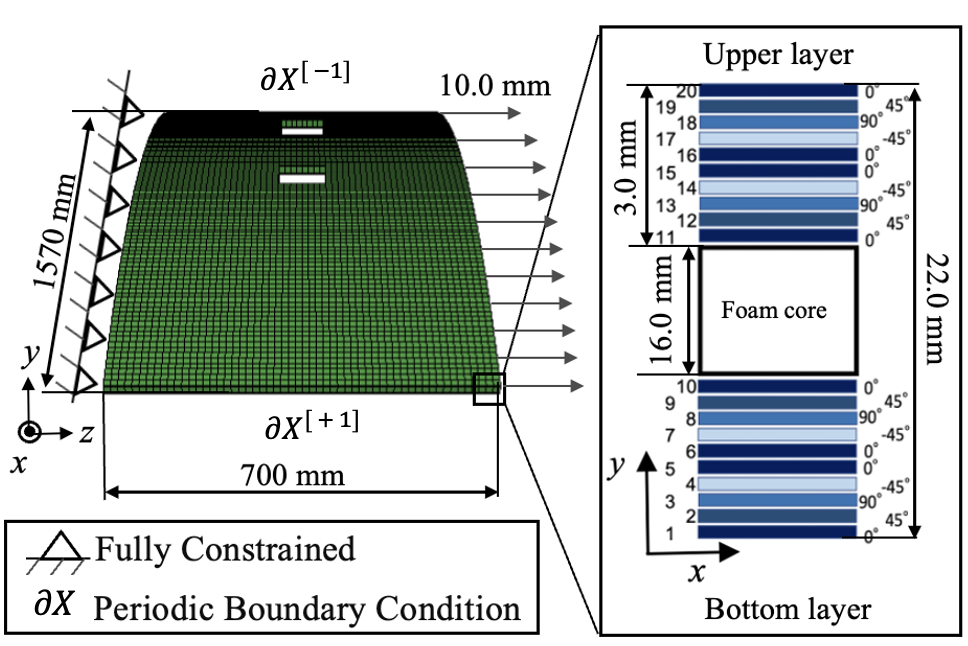
\includegraphics[width=\linewidth]{fem_condition.png}\\
  {\scriptsize Perforated CFRP interstage panel (FEM).}
\end{column}
\end{columns}
\end{frame}

% ---------------------------------------------------------------------
\begin{frame}{Infrared stress measurement (DSPSS)}
\begin{columns}[T]
\begin{column}{0.55\textwidth}
Thermoelastic effect relates a small temperature change to the change in
the sum of principal stresses:
\[
  \Delta T = -k\,T\,\Delta\sigma_{\mathrm{sum}},\qquad
  \sigma_{\mathrm{sum}} = \sigma_1+\sigma_2+\sigma_3 = \mathrm{tr}(\boldsymbol\sigma).
\]
Infrared stress measurement~\cite{ir1_main,ir1,sakagami2016} thus yields a
\textbf{full-field surface map} of $\sigma_{\mathrm{sum}}$ (DSPSS), from which
sub-surface defects are inferred.
\end{column}
\begin{column}{0.45\textwidth}
  \centering
  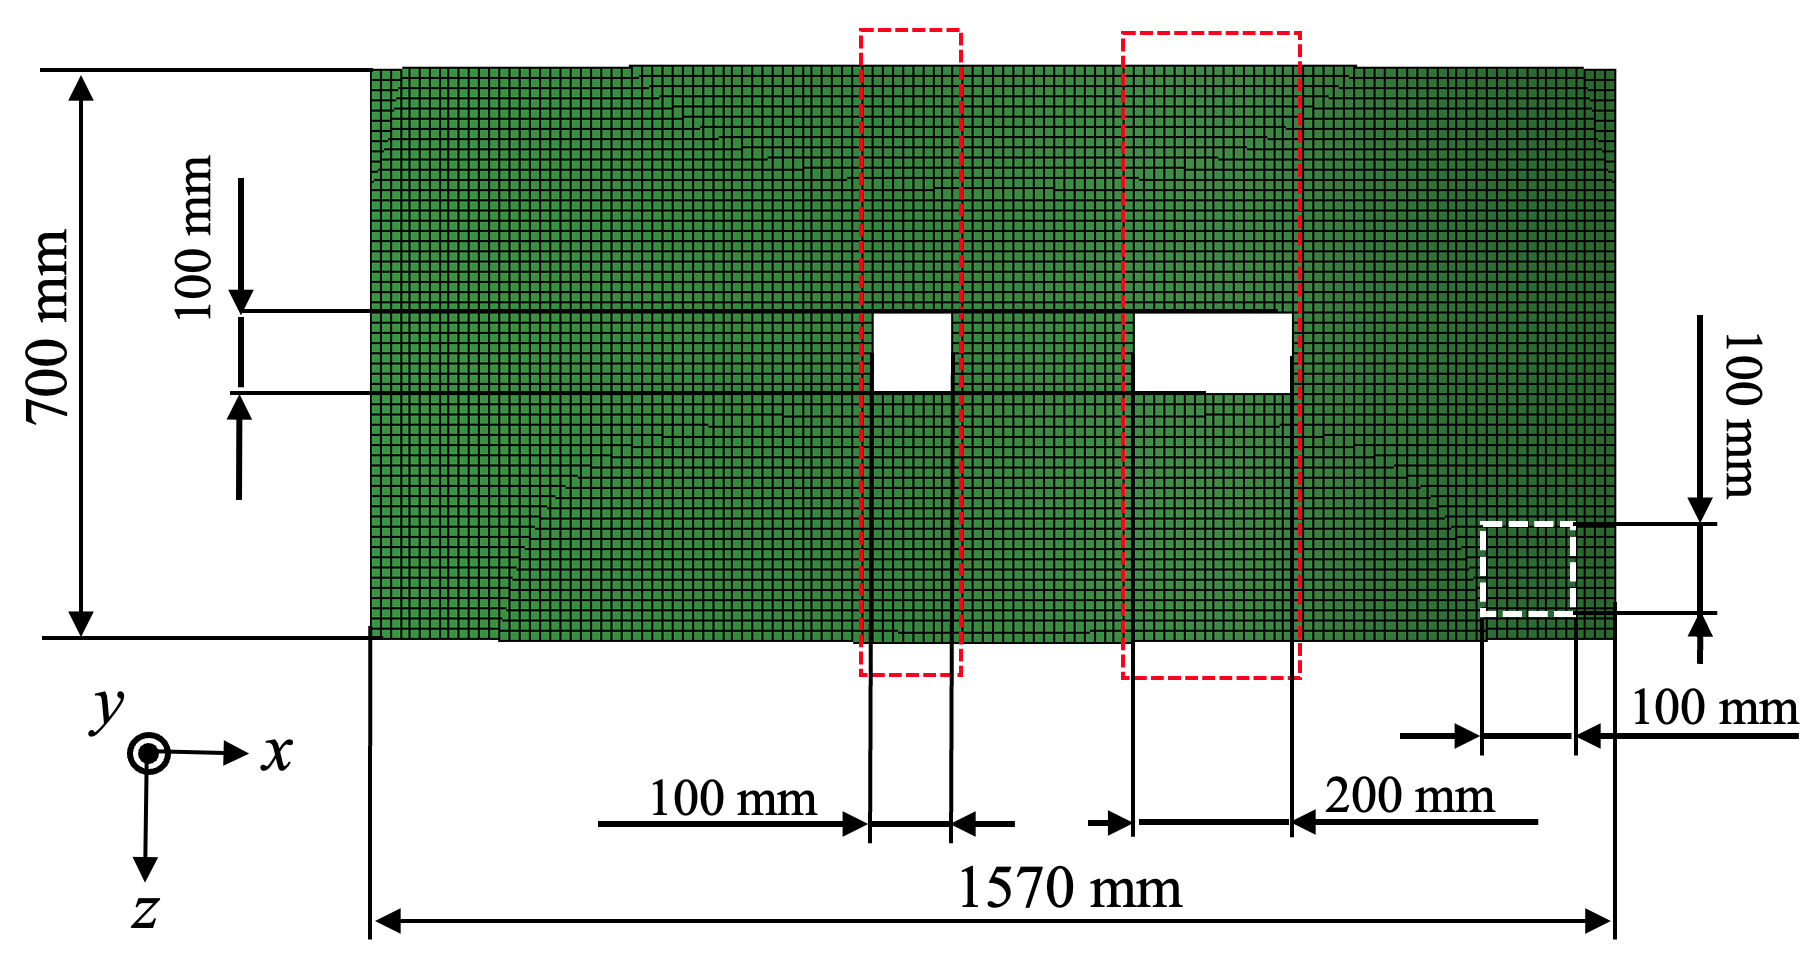
\includegraphics[width=\linewidth]{dspss_defect.png}\\
  {\scriptsize DSPSS shows a stress valley over the defect.}
\end{column}
\end{columns}
\end{frame}

% ---------------------------------------------------------------------
\begin{frame}{Previous study and purpose}
\begin{itemize}
  \item \textbf{Previous study}~\cite{kojima,kojima2024_transfer}:
        transfer learning with a CNN estimates defect position/size — but is
        tied to image grids and struggles on irregular, perforated geometry.
  \item \textbf{This work}: a \textbf{Graph Neural Network} (GAT) that
        consumes FEM-generated DSPSS to predict the \emph{3-D defect location}
        (in-plane region $\times$ insertion layer) in perforated CFRP interstage
        structures.
\end{itemize}
\vspace{0.4em}
\begin{block}{Why a graph?}
The FEM surface mesh is naturally a graph; a GNN handles the irregular,
hole-perforated topology that a CNN grid cannot.
\end{block}
\end{frame}

% ---------------------------------------------------------------------
\begin{frame}{FEM analysis conditions}
\begin{columns}[T]
\begin{column}{0.54\textwidth}
\begin{itemize}
  \item $1/80$-scale curved panel ($R\approx 2$\,m, $L\approx 1.57$\,m, $t=22$\,mm).
  \item Holes of $100\times100$ and $200\times100$\,mm.
  \item Sandwich laminate; tensile loading.
  \item Interlaminar delamination modeled explicitly by \textbf{Teflon inserts}
        between selected plies.
\end{itemize}
\vspace{0.3em}
Synthetic dataset $\Rightarrow$ DSPSS fields with known ground-truth defects.
\end{column}
\begin{column}{0.46\textwidth}
  \centering
  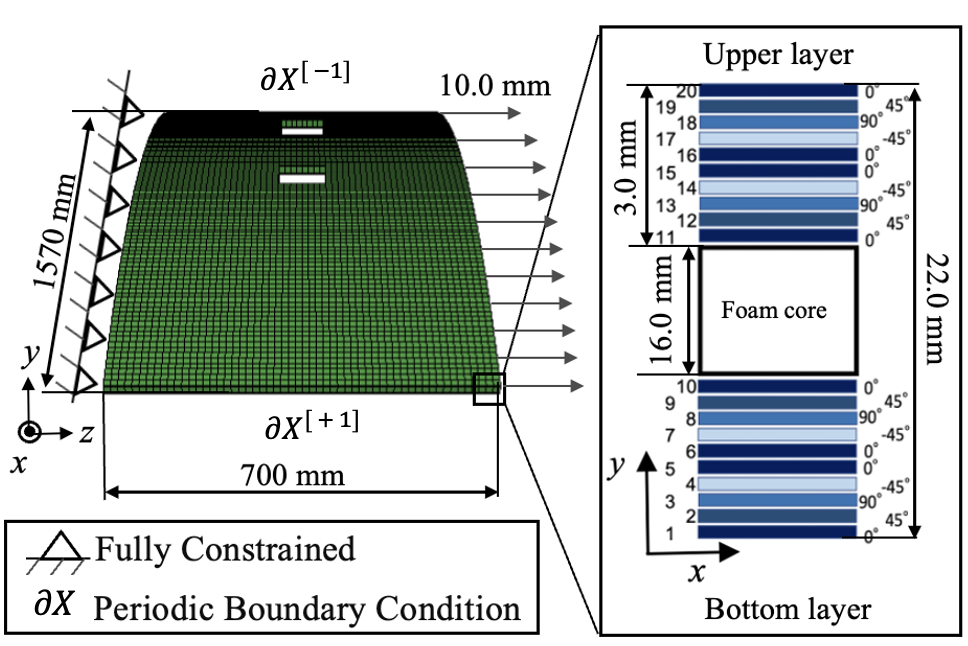
\includegraphics[width=\linewidth]{fem_condition.png}\\
  {\scriptsize FEM boundary conditions \& hole geometry.}
\end{column}
\end{columns}
\end{frame}

% ---------------------------------------------------------------------
\begin{frame}{Input data: normalized / difference DSPSS}
\begin{columns}[T]
\begin{column}{0.52\textwidth}
Raw DSPSS is dominated by \textbf{stress concentration around the hole},
masking the defect signal.

\vspace{0.5em}
Remedy (paper):
\begin{itemize}
  \item \textbf{Difference} field: damaged $-$ defect-free reference;
  \item \textbf{Z-score normalization} (per node), improving depth-direction
        discrimination.
\end{itemize}
\vspace{0.4em}
$\Rightarrow$ robust localization even near the opening.
\end{column}
\begin{column}{0.48\textwidth}
  \centering
  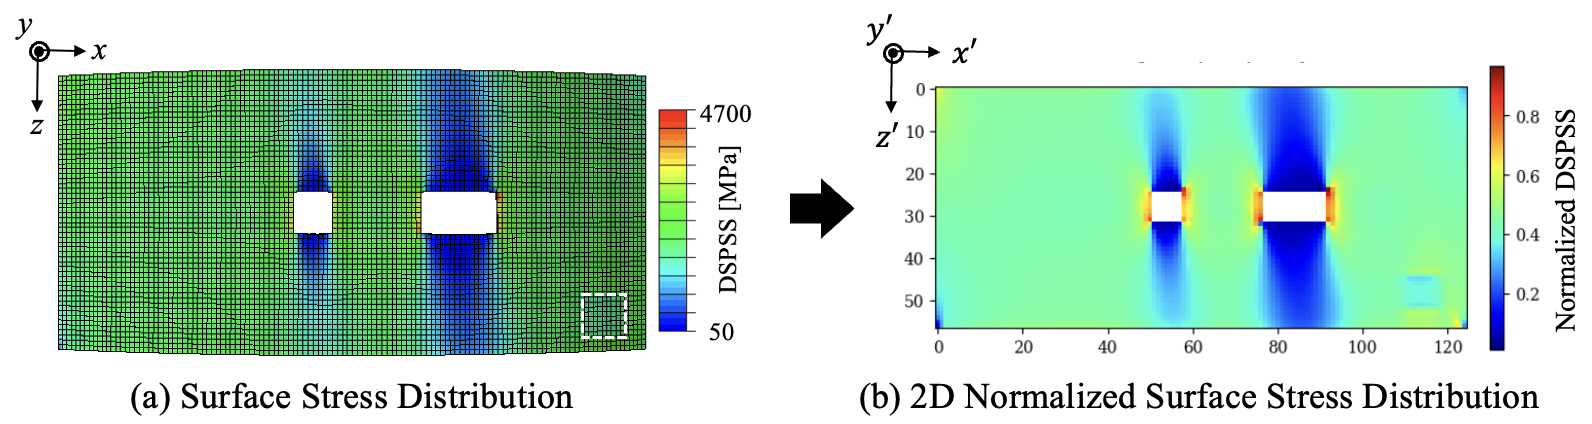
\includegraphics[width=\linewidth]{dspss_normalized.png}\\
  {\scriptsize Normalized DSPSS isolates the defect.}
\end{column}
\end{columns}
\end{frame}

% ---------------------------------------------------------------------
\begin{frame}{Stress distribution around the defect}
\begin{itemize}
  \item DSPSS exhibits a clear \textbf{stress valley} at the defect centre.
  \item Depth and width of the valley depend on \textbf{ply angle}:
        $90^\circ$ plies give sharp narrow valleys; $0^\circ/45^\circ$ broaden them.
  \item This ply-angle signature is what the network must learn to separate
        \emph{which layer} the delamination sits in.
\end{itemize}
\vspace{0.5em}
\begin{exampleblock}{Implication}
Layer discrimination is a \emph{fine spatial-frequency} problem — motivating
attention over local neighbourhoods.
\end{exampleblock}
\end{frame}

% ---------------------------------------------------------------------
\begin{frame}{Graph representation \& GAT model}
\begin{columns}[T]
\begin{column}{0.5\textwidth}
\begin{itemize}
  \item \textbf{Nodes} = FEM surface elements;
        features $=(x,y,z,\hat\sigma_{\mathrm{sum}})$.
  \item \textbf{Edges} = fixed mesh connectivity (reused across graphs).
  \item \textbf{GAT}~\cite{gat1,gnn1}: attention weights learn neighbour
        importance; message passing~\cite{gilmer2017mpnn} over the mesh.
  \item Architecture: $3\times$ GATConv ($64{\to}256{\to}256$), multi-head,
        batch-norm + dropout + residual connections.
\end{itemize}
\end{column}
\begin{column}{0.5\textwidth}
  \centering
  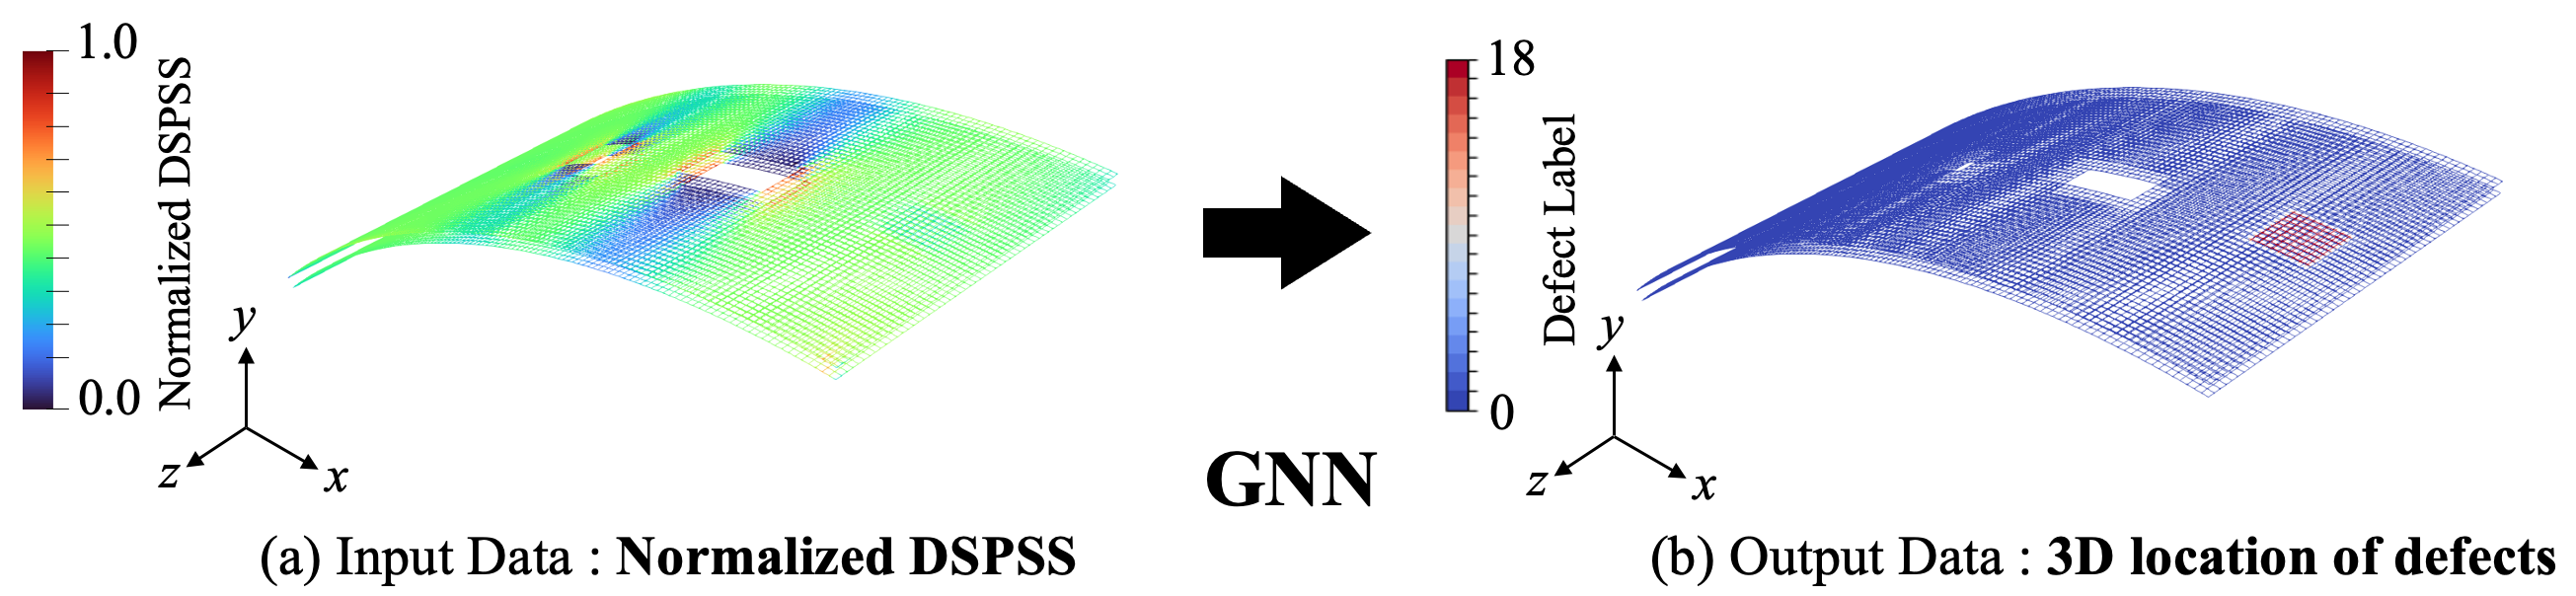
\includegraphics[width=\linewidth]{gnn_model.png}\\
  {\scriptsize Graph model on the perforated mesh.}
\end{column}
\end{columns}
\end{frame}

% ---------------------------------------------------------------------
\begin{frame}{Output: 3-D defect location as 19-class node labels}
\begin{columns}[T]
\begin{column}{0.52\textwidth}
\begin{itemize}
  \item Node classification into \textbf{19 classes}:
        class 0 $=$ defect-free; remaining classes encode
        \emph{in-plane region} $\times$ \emph{insertion layer}.
  \item One-side labelling so prediction needs only single-surface DSPSS.
\end{itemize}
\vspace{0.4em}
\begin{block}{Severe imbalance}
Defect nodes are $<3\%$ of all nodes — handled by the loss (next slide).
\end{block}
\end{column}
\begin{column}{0.48\textwidth}
  \centering
  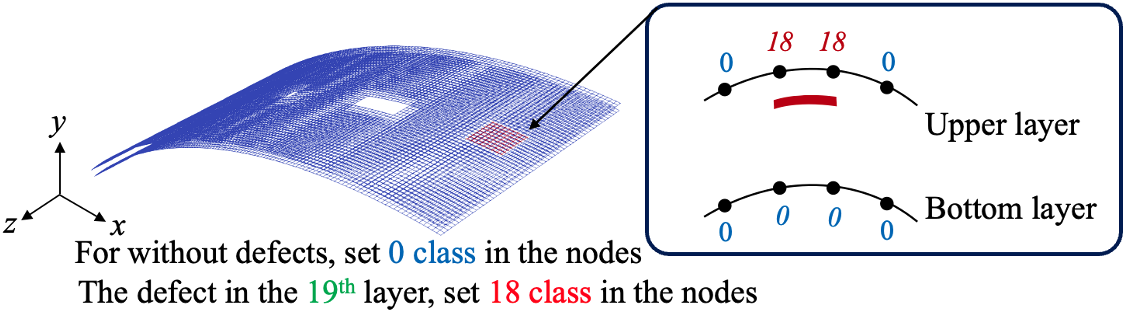
\includegraphics[width=\linewidth]{label19.png}\\
  {\scriptsize 19-class label map.}
\end{column}
\end{columns}
\end{frame}

% ---------------------------------------------------------------------
\begin{frame}{Loss function: Focal loss}
\[
  \mathrm{FL}(p_t) = -\,\alpha_t\,(1-p_t)^{\gamma}\,\log p_t .
\]
\begin{itemize}
  \item Down-weights easy, abundant defect-free nodes;
        emphasises rare defect-class nodes~\cite{focal_loss}.
  \item Crucial because intact regions dominate ($>97\%$).
\end{itemize}
\vspace{0.4em}
Node features normalized; a single fixed edge list reused across all graphs.
\end{frame}

% ---------------------------------------------------------------------
\begin{frame}{Results: prediction accuracy}
\begin{columns}[T]
\begin{column}{0.5\textwidth}
Test-set metrics:
\begin{itemize}
  \item planar $R = 0.72$ (mean), depth $P_{\mathrm{gauss}} = 0.69$,
        combined $\mathrm{TDPS} = 0.70$ (best $0.92$).
  \item Best layers: 9--12 (mid-thickness); Layer-10 samples all
        $\mathrm{TDPS}\ge 0.82$.
  \item False-negative rate for defect nodes \textbf{$<3\%$}.
\end{itemize}
\end{column}
\begin{column}{0.5\textwidth}
  \centering
  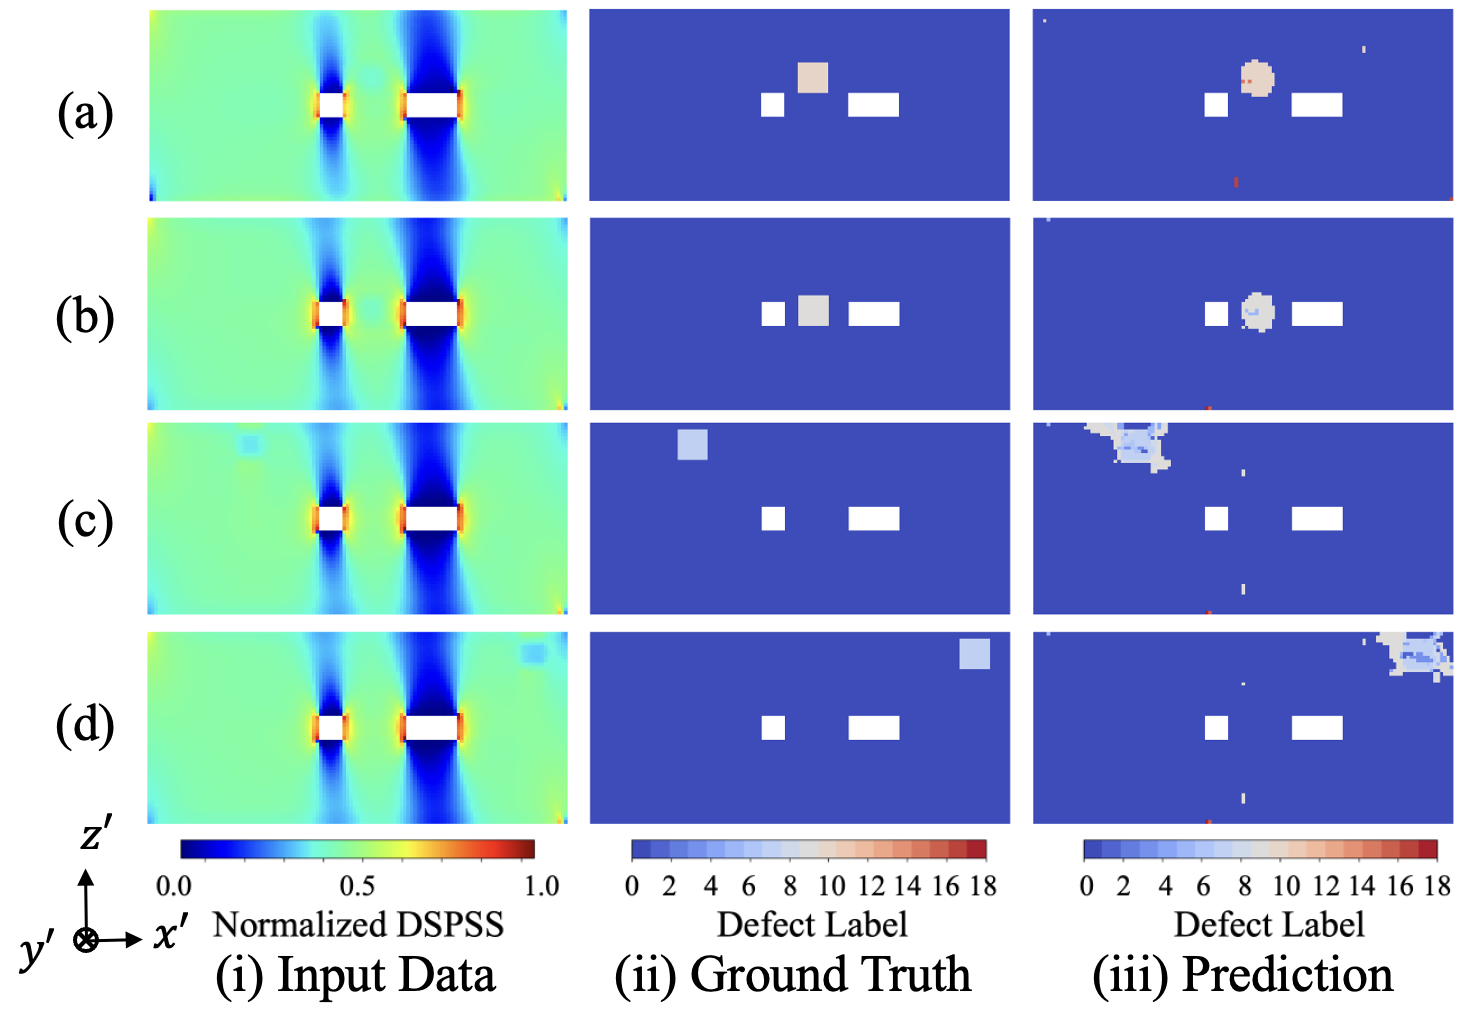
\includegraphics[height=0.34\textheight]{pred_l4.png}\\
  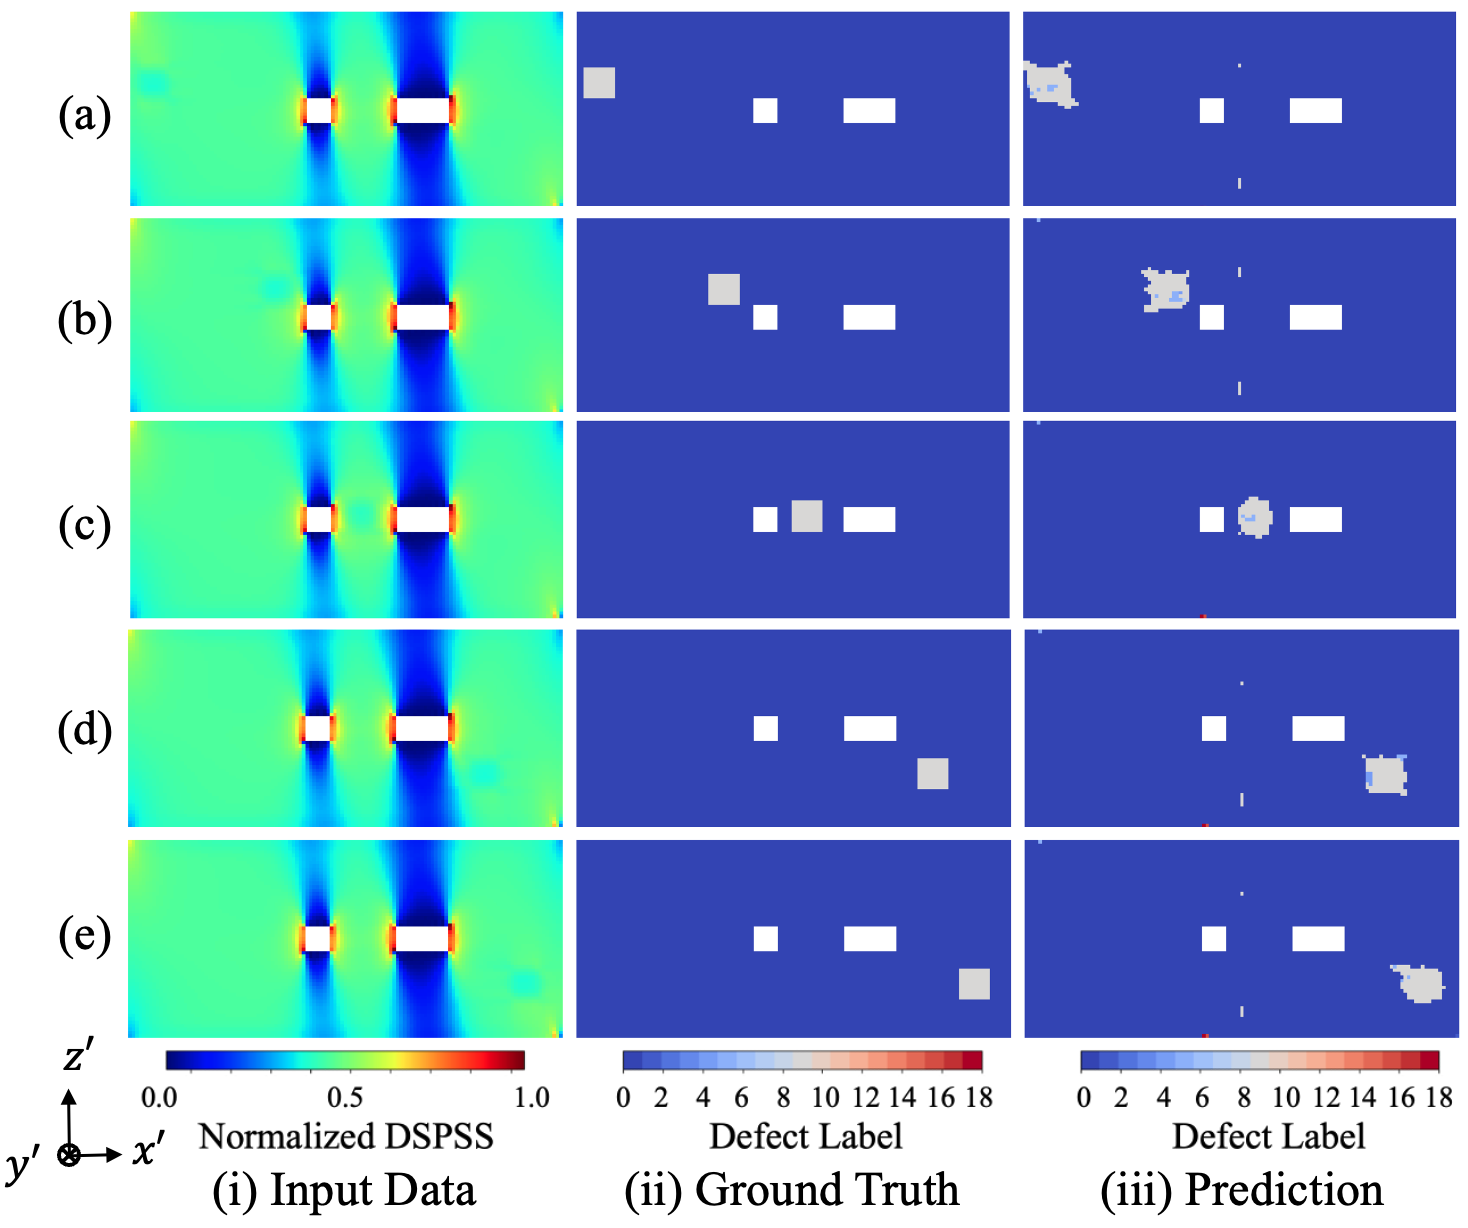
\includegraphics[height=0.34\textheight]{pred_l10.png}\\
  {\scriptsize Predicted vs.\ true defect regions.}
\end{column}
\end{columns}
\end{frame}

% ---------------------------------------------------------------------
\begin{frame}{Overall performance \& confusion}
\begin{columns}[T]
\begin{column}{0.5\textwidth}
  \begin{block}{Headline}
  \best{Macro-F1 $= 61\%$} across 19 classes, using \emph{surface DSPSS only}.
  \end{block}
  \begin{itemize}
    \item Dominant diagonal; residual \emph{adjacent-layer} confusion.
    \item False positives cluster near the hole edge.
    \item Robust across defect insertion regions.
  \end{itemize}
\end{column}
\begin{column}{0.5\textwidth}
  \centering
  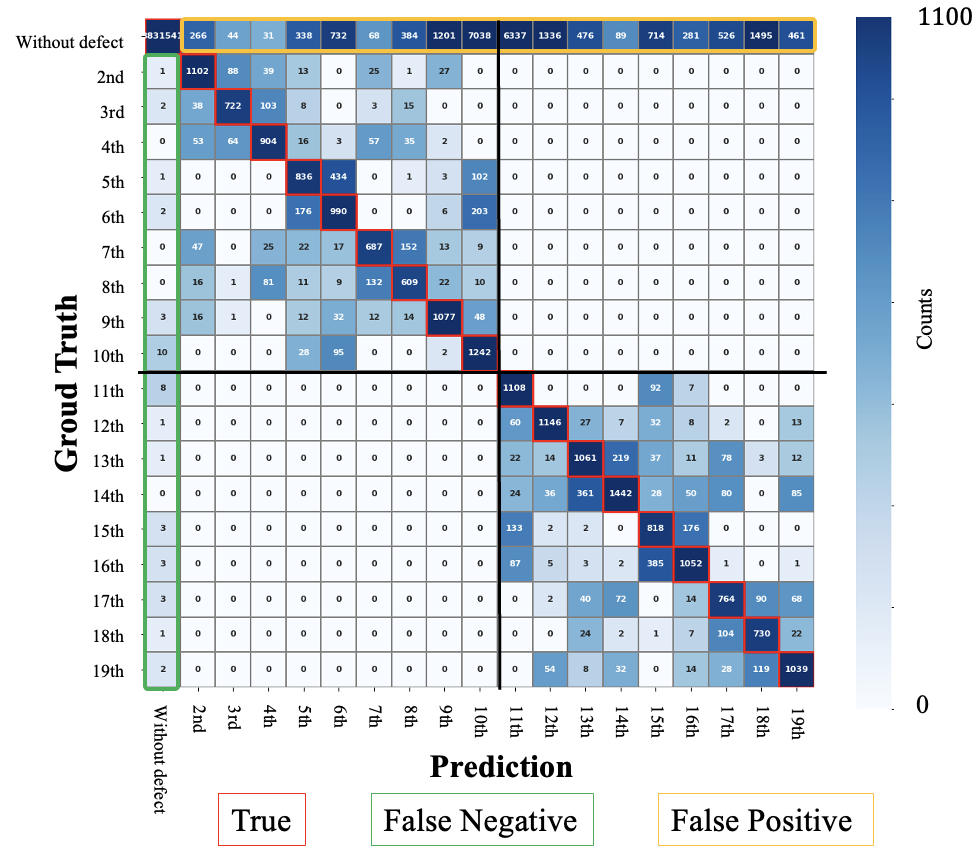
\includegraphics[width=\linewidth]{confusion_61.png}\\
  {\scriptsize Confusion matrix (macro-F1 61\%).}
\end{column}
\end{columns}
\end{frame}

% ---------------------------------------------------------------------
\begin{frame}{Conclusion}
\begin{itemize}
  \item Introduced an \textbf{FEM + GAT} framework for 3-D delamination
        localization in perforated CFRP interstage panels.
  \item \textbf{Difference-normalized DSPSS} suppresses hole stress
        concentration and enables full-region estimation.
  \item Achieved \best{macro-F1 $61\%$} on 19 classes from surface data only,
        with a very low defect false-negative rate and no false detections in
        defect-free regions.
\end{itemize}
\vspace{0.3em}
\begin{block}{A scalable foundation}
toward experimental infrared-stress (TSA) data and practical SHM of aerospace
composite structures.
\end{block}
\end{frame}

% =====================================================================
%  NEW CONTRIBUTION (beyond last year's paper): noise robustness + NDF.
%  This is exactly the WCCM-abstract delta ("robustness under
%  experimentally motivated noise conditions") — co-author-vetted.
% =====================================================================
\begin{frame}{New focus: robustness for real operation}
\begin{columns}[T]
\begin{column}{0.55\textwidth}
The published model assumes clean FEM fields. In practice:
\begin{itemize}
  \item infrared stress measurement carries \textbf{acquisition noise}
        (temperature fluctuation, emissivity, sensor);
  \item the vast majority of a real structure is \textbf{defect-free} — false
        detections there are costly.
\end{itemize}
\vspace{0.4em}
\begin{alertblock}{WCCM contribution}
Train for \emph{robustness under experimentally-motivated noise} and explicitly
\emph{suppress false detection} on defect-free regions.
\end{alertblock}
\end{column}
\begin{column}{0.45\textwidth}
  \centering
  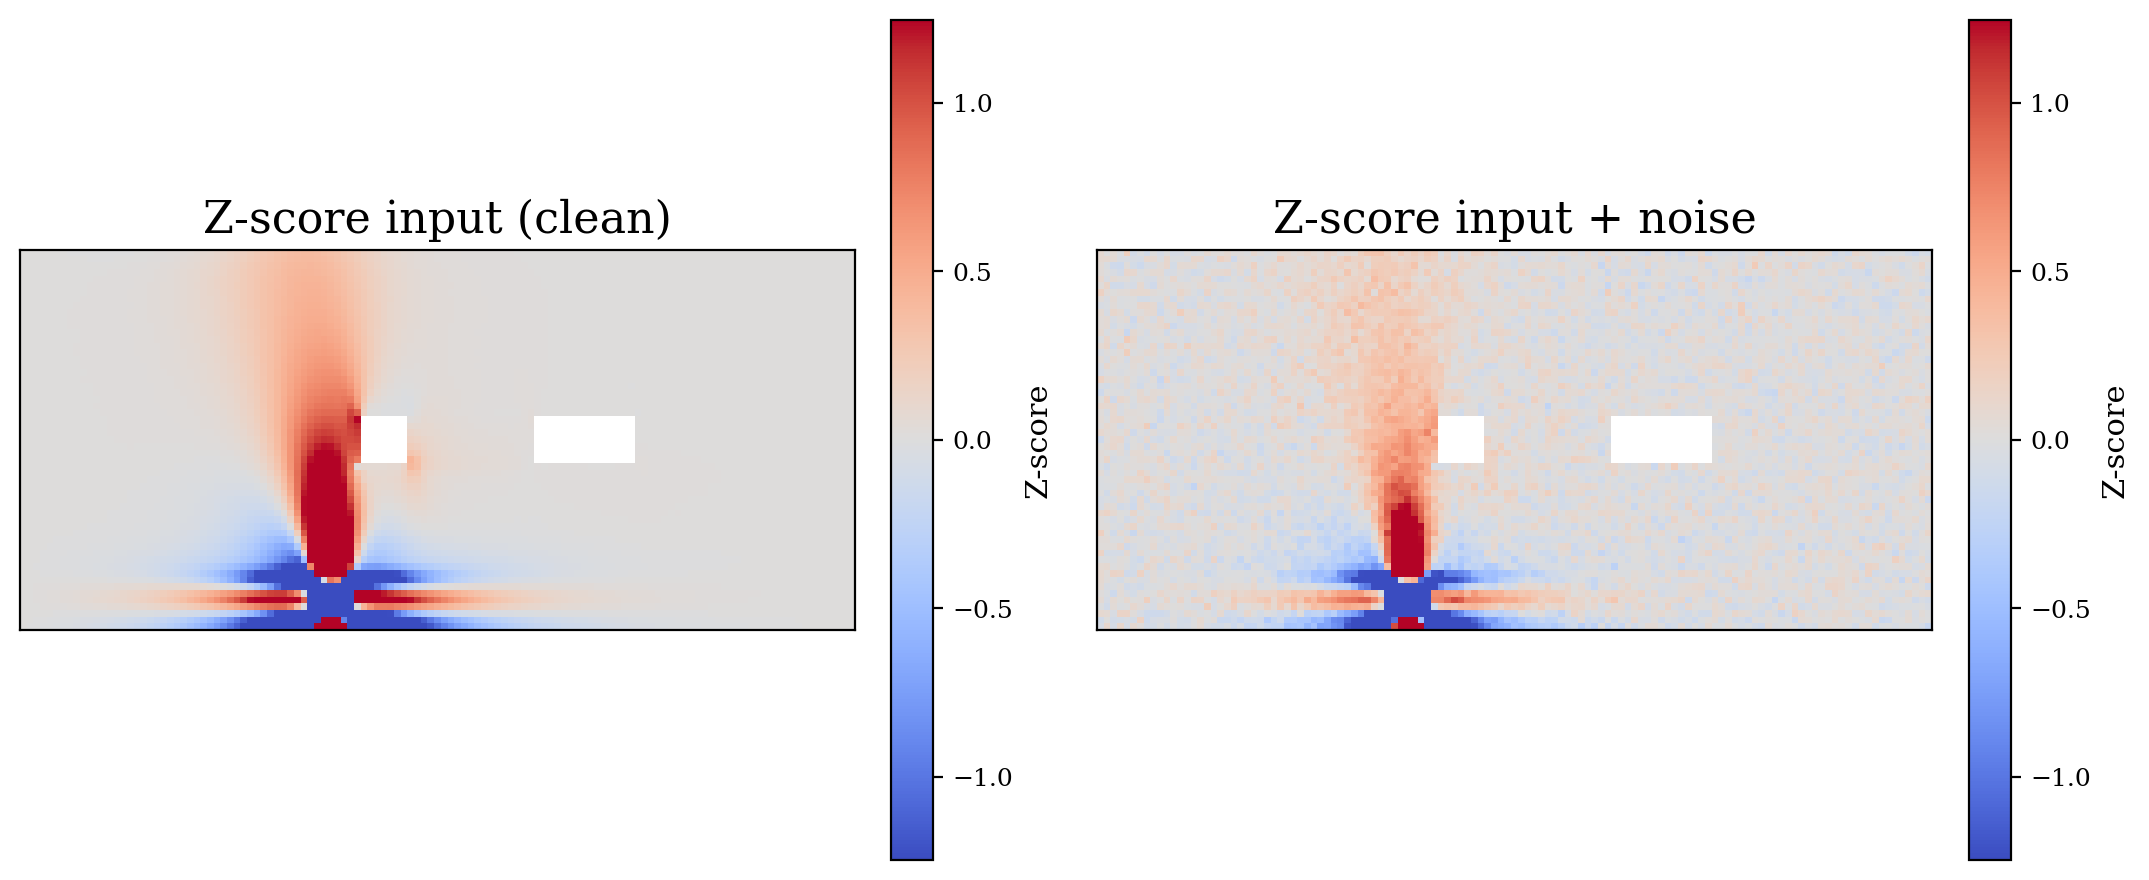
\includegraphics[width=\linewidth]{noise_clean.png}\\
  {\scriptsize Clean vs.\ noise-injected Z-score input — the defect signature survives.}
\end{column}
\end{columns}
\end{frame}

% ---------------------------------------------------------------------
\begin{frame}{Noise-augmented dataset \& defect-free negatives (NDF)}
\begin{columns}[T]
\begin{column}{0.52\textwidth}
\textbf{Defect-free negatives (NDF):}
\begin{itemize}
  \item base field set to zero (no defect);
  \item additive Gaussian noise ($10\%$ of data std);
  \item $5{,}000$ samples added to training.
\end{itemize}
\textbf{Noise model on defect data:}
\begin{itemize}
  \item line noise along the fibre ($z$) direction (random intensity/width);
  \item attenuated noise in $x$; global white noise.
\end{itemize}
\end{column}
\begin{column}{0.48\textwidth}
  \centering
  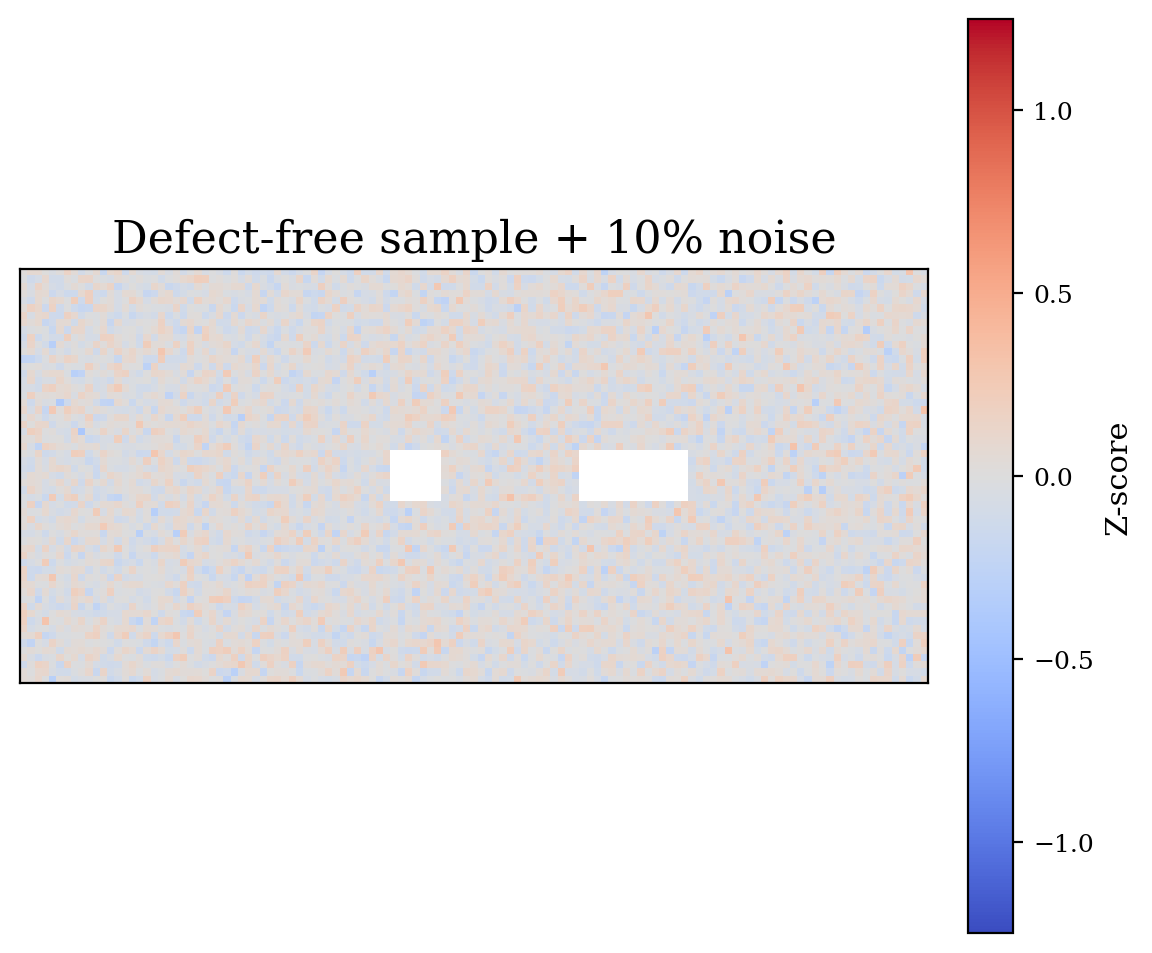
\includegraphics[width=\linewidth]{ndf_clean.png}\\
  {\scriptsize A defect-free sample (zero field $+$ 10\% noise) — teaches ``no defect''.}
\end{column}
\end{columns}
\end{frame}

% ---------------------------------------------------------------------
\begin{frame}{Results under noise}
\begin{columns}[T]
\begin{column}{0.5\textwidth}
\begin{itemize}
  \item Difference-DSPSS input enables \textbf{full-region} defect estimation.
  \item Prediction stays accurate on \textbf{noise-injected} data.
  \item \textbf{No false detection} on defect-free inputs — the NDF negatives
        remove spurious activations.
\end{itemize}
\vspace{0.4em}
\begin{block}{Takeaway}
The framework is robust enough to move toward \emph{experimental} infrared
stress data.
\end{block}
\end{column}
\begin{column}{0.5\textwidth}
  \centering
  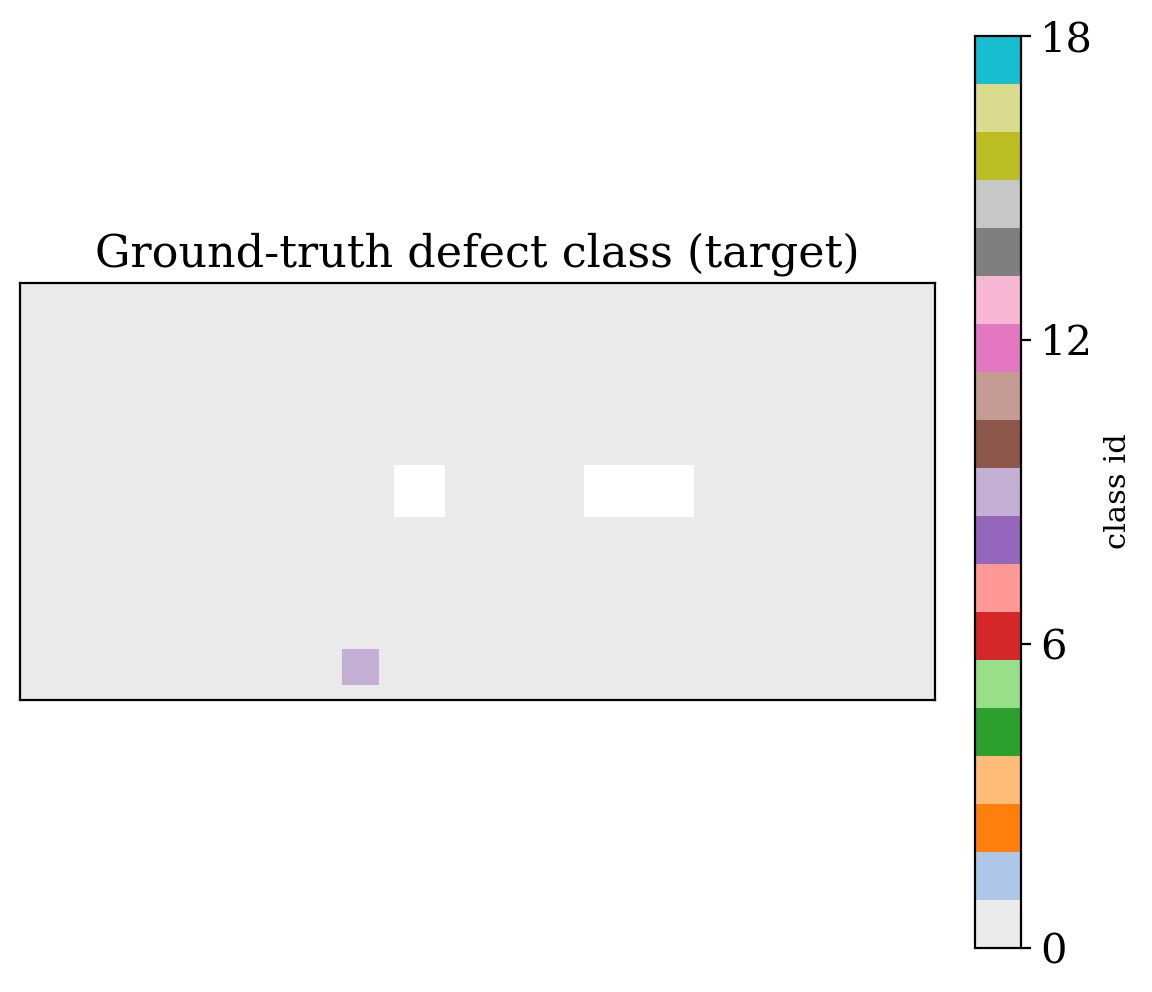
\includegraphics[width=\linewidth]{label_clean.png}\\
  {\scriptsize Ground-truth defect class to be localized (target).}
\end{column}
\end{columns}
\end{frame}

% ---------------------------------------------------------------------
\begin{frame}{Outlook \quad {\small[ongoing, beyond the published paper]}}
\begin{itemize}
  \item \textbf{Sim-to-real:} apply the noise-robust model to \emph{experimental}
        infrared-stress (TSA) measurements.
  \item \textbf{Architecture study (preliminary):} extending from attention
        GNNs to \emph{mesh-physics} GNNs (MeshGraphNet) and layered variants;
        early results are encouraging and under evaluation with co-authors.
  \item \textbf{Application:} transfer to aerospace payload-fairing SHM.
\end{itemize}
\vspace{0.3em}
{\footnotesize\itshape Preliminary; not part of the published results.}
\end{frame}

% ---------------------------------------------------------------------
\begin{frame}[allowframebreaks]{References}
\renewcommand*{\bibfont}{\scriptsize}
\printbibliography[heading=none]
\end{frame}

% =====================================================================
%  APPENDIX — difference-data details (course-1 / 差分データ)
% =====================================================================
\appendix

\begin{frame}[standout]
Appendix
\end{frame}

% ---------------------------------------------------------------------
\begin{frame}{Appendix: difference-data construction}
\begin{columns}[T]
\begin{column}{0.5\textwidth}
Raw DSPSS near a hole is dominated by geometric stress concentration.
We remove it by a per-specimen \textbf{difference}:
\[
  \text{Difference} = \underbrace{\text{Original (defect)}}_{\text{damaged}}
  - \underbrace{\text{Reference (no defect)}}_{\text{pristine}} .
\]
The residual isolates the defect-induced perturbation, independent of the
hole's baseline field.
\end{column}
\begin{column}{0.5\textwidth}
  \centering
  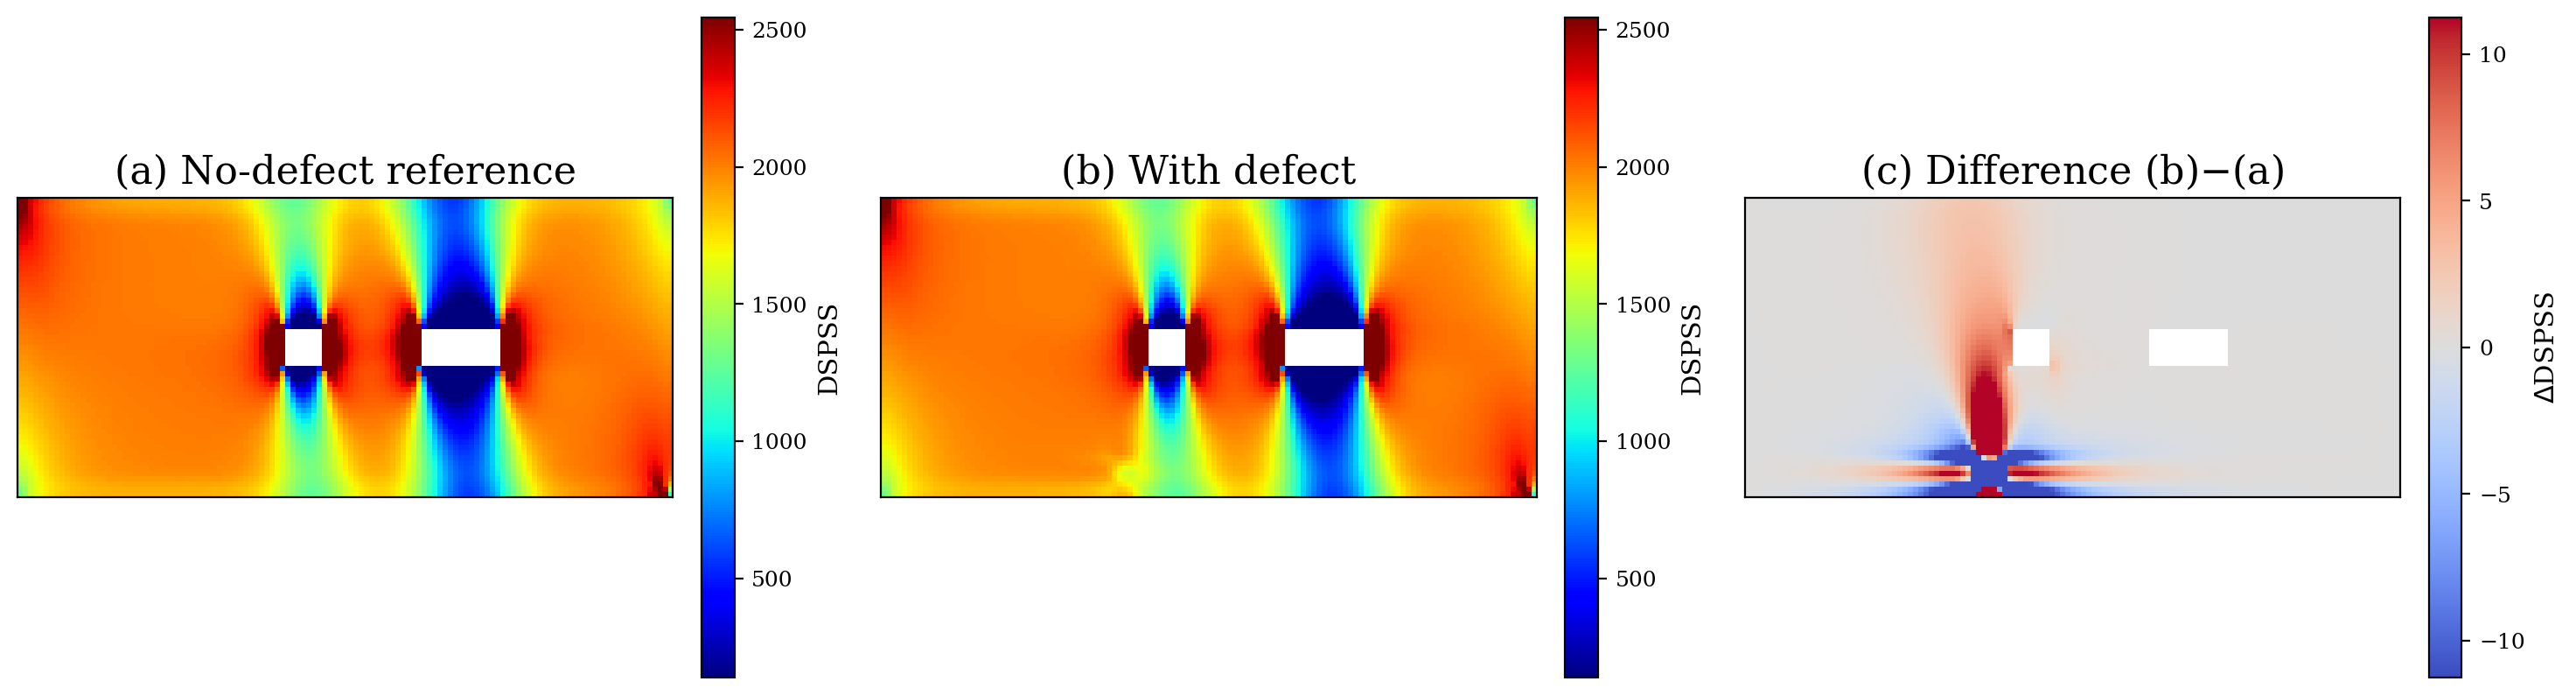
\includegraphics[width=\linewidth]{diff_clean.png}\\
  {\scriptsize With-defect $-$ no-defect reference $=$ difference field (defect localized).}
\end{column}
\end{columns}
\end{frame}

% ---------------------------------------------------------------------
\begin{frame}{Appendix: Z-score normalization}
\begin{columns}[T]
\begin{column}{0.5\textwidth}
The difference field is standardized per node (Z-score):
\[
  \hat\sigma = \frac{\sigma - \mu}{s}.
\]
\begin{itemize}
  \item equalizes magnitude across regions/specimens;
  \item improves \textbf{depth-direction} (layer) discrimination;
  \item keeps the network NDT-admissible (coordinate/stress only).
\end{itemize}
\end{column}
\begin{column}{0.5\textwidth}
  \centering
  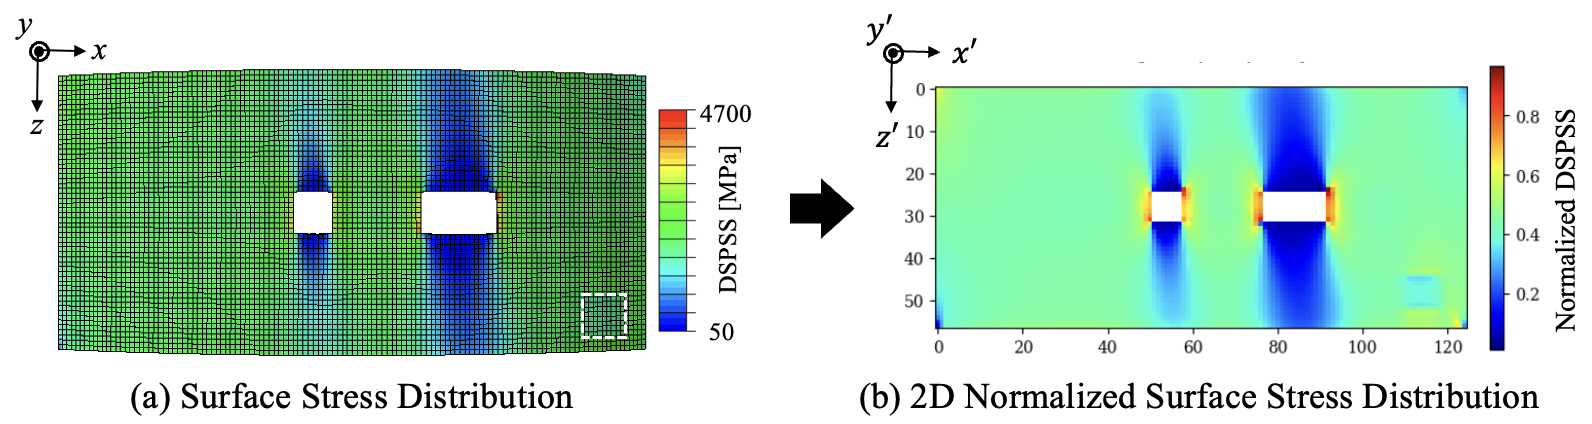
\includegraphics[width=\linewidth]{dspss_normalized.png}\\
  {\scriptsize Normalized DSPSS input (paper figure).}
\end{column}
\end{columns}
\end{frame}

% ---------------------------------------------------------------------
\begin{frame}{Appendix: DSPSS profile around the defect}
\begin{columns}[T]
\begin{column}{0.46\textwidth}
The difference-DSPSS shows a pronounced \textbf{stress valley} at the defect
centre; its depth and width encode the insertion layer (ply-angle dependence).
\end{column}
\begin{column}{0.54\textwidth}
  \centering
  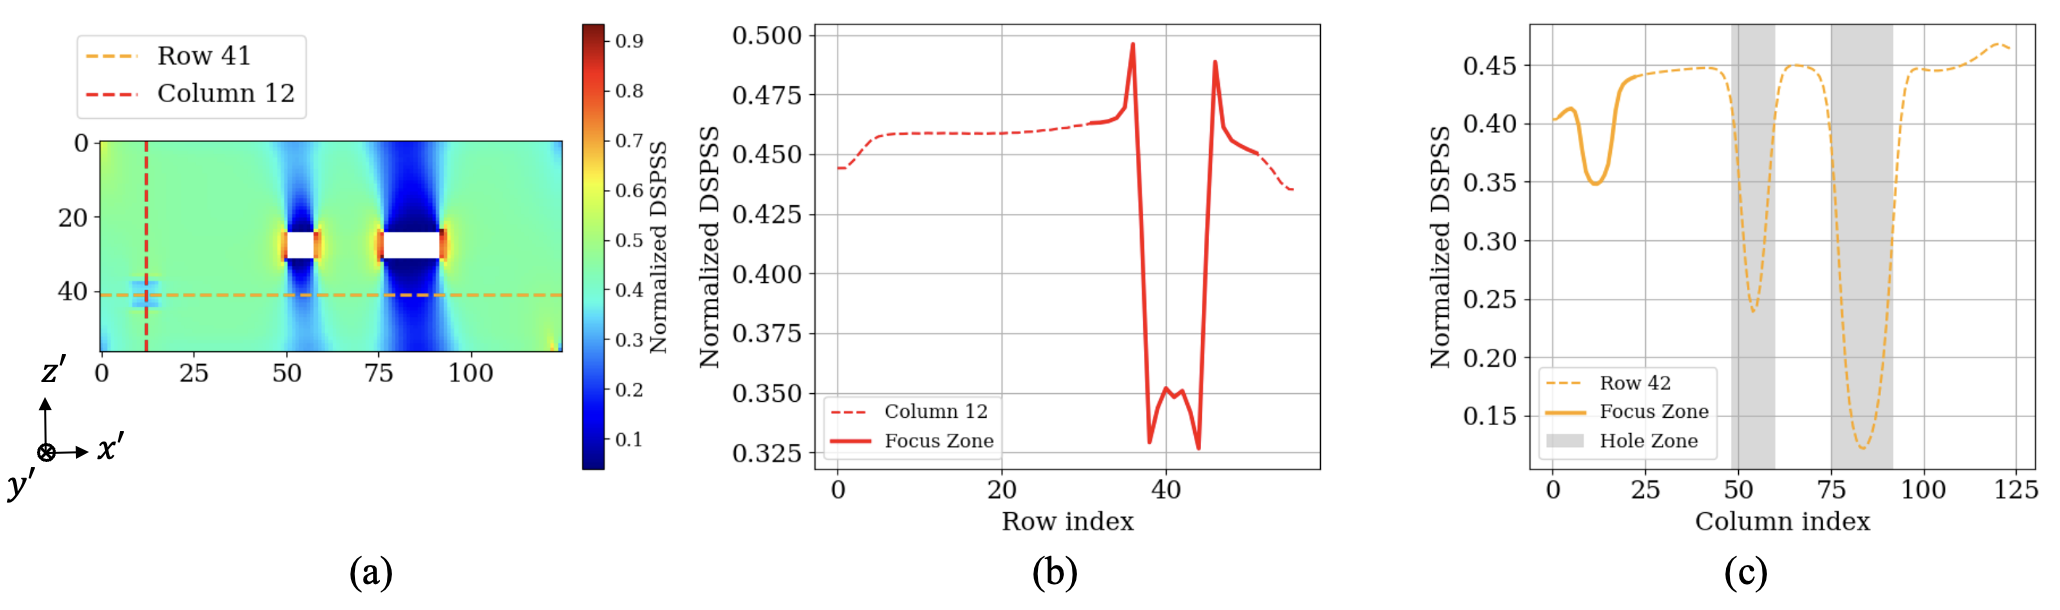
\includegraphics[width=\linewidth]{dspss_profile.png}\\
  {\scriptsize Profile of the normalized DSPSS across the defect (paper figure).}
\end{column}
\end{columns}
\end{frame}

\end{document}
